\documentclass[12pt]{beamer}
% You can use \documentclass[11pt,aspectratio=169]{beamer} 
% to adjust the aspect ratio to 16:9.

\renewcommand{\figurename}{}
\renewcommand{\tablename}{}
\renewcommand\thefigure{\arabic{figure} pav.}
\renewcommand\thetable{\arabic{table} lentelė.}

\usepackage{graphicx}
\usepackage{listings}
\usepackage[
	backend=biber,
	style=numeric,
	sorting=ynt
]{biblatex}
\usepackage{algorithm,algorithmic}
\usepackage{caption}
\usepackage{subfig}

\usepackage{biblatex}
\usepackage{hyperref}
\usepackage{makecell}

\addbibresource{references.bib}

\usetheme{Madrid}

\title[]{Programų, skirtų prekiauti kripto valiutas, kūrimas, tobulinimas ir testavimas, naudojant Go ir Rust programavimo kalbas}
\subtitle[]{Profesinės praktikos ataskaita}
\author[Vismantas Stonkus]{Vismantas Stonkus}
\date{}

\addtobeamertemplate{author}{}{VU praktikos vadovas: Prof. dr. Remigijus Paulavičius\par}
\addtobeamertemplate{author}{}{Išorinis praktikos vadovas: Marius Baškys\par}

\setbeamertemplate{navigation symbols}{}

\usepackage{VUMIF}

\begin{document}

\begin{frame}
    \titlepage
\end{frame}

\begin{frame}{Įmonė - Humbility UAB}
yra pirma didelės apimties kriptovaliutų prekybos įmonė, specializuojanti arbitražo operacijose tarp įvairių biržų.

\begin{figure}[H]
  \centering
  
\includegraphics[scale=0.2]{resources/site.png}
  \caption{Įmonės puslapis. https://humbility.io}
  \label{img:site}
\end{figure}
\end{frame}

\begin{frame}{Įmonės veikla}
Įmonė veikia tiek centralizuotose (CEX), tiek decentralizuotose (DEX) kriptovaliutų biržose.
  % centralizuotos platformos veikia pagal tradicini finansu modeli. t.y. jos turi centra, kuris valdo ir kontroliuoja prekybos procesa,
  % kur decentralizuotos platformos leidzia vartotojas tiesiogiai keistis kriptovaliutomis naudojant ismaniuosius kontraktus ir bloku grandine.
  % as praktika atlikau komandoje kuri specializuojasi tik dex'uose
  % Is situ punktu ka imone veikia mano komandai atitinkai tik kaireje
  % t.y. mes renkame ir analizuojame didelius kiekius rinkos duomenu
  % Implementuojame modelius prekiauti rinkoje efektyviai.
  % Ir leidziame auksto daznio prekyba

  \begin{figure}[H]
    \centering
    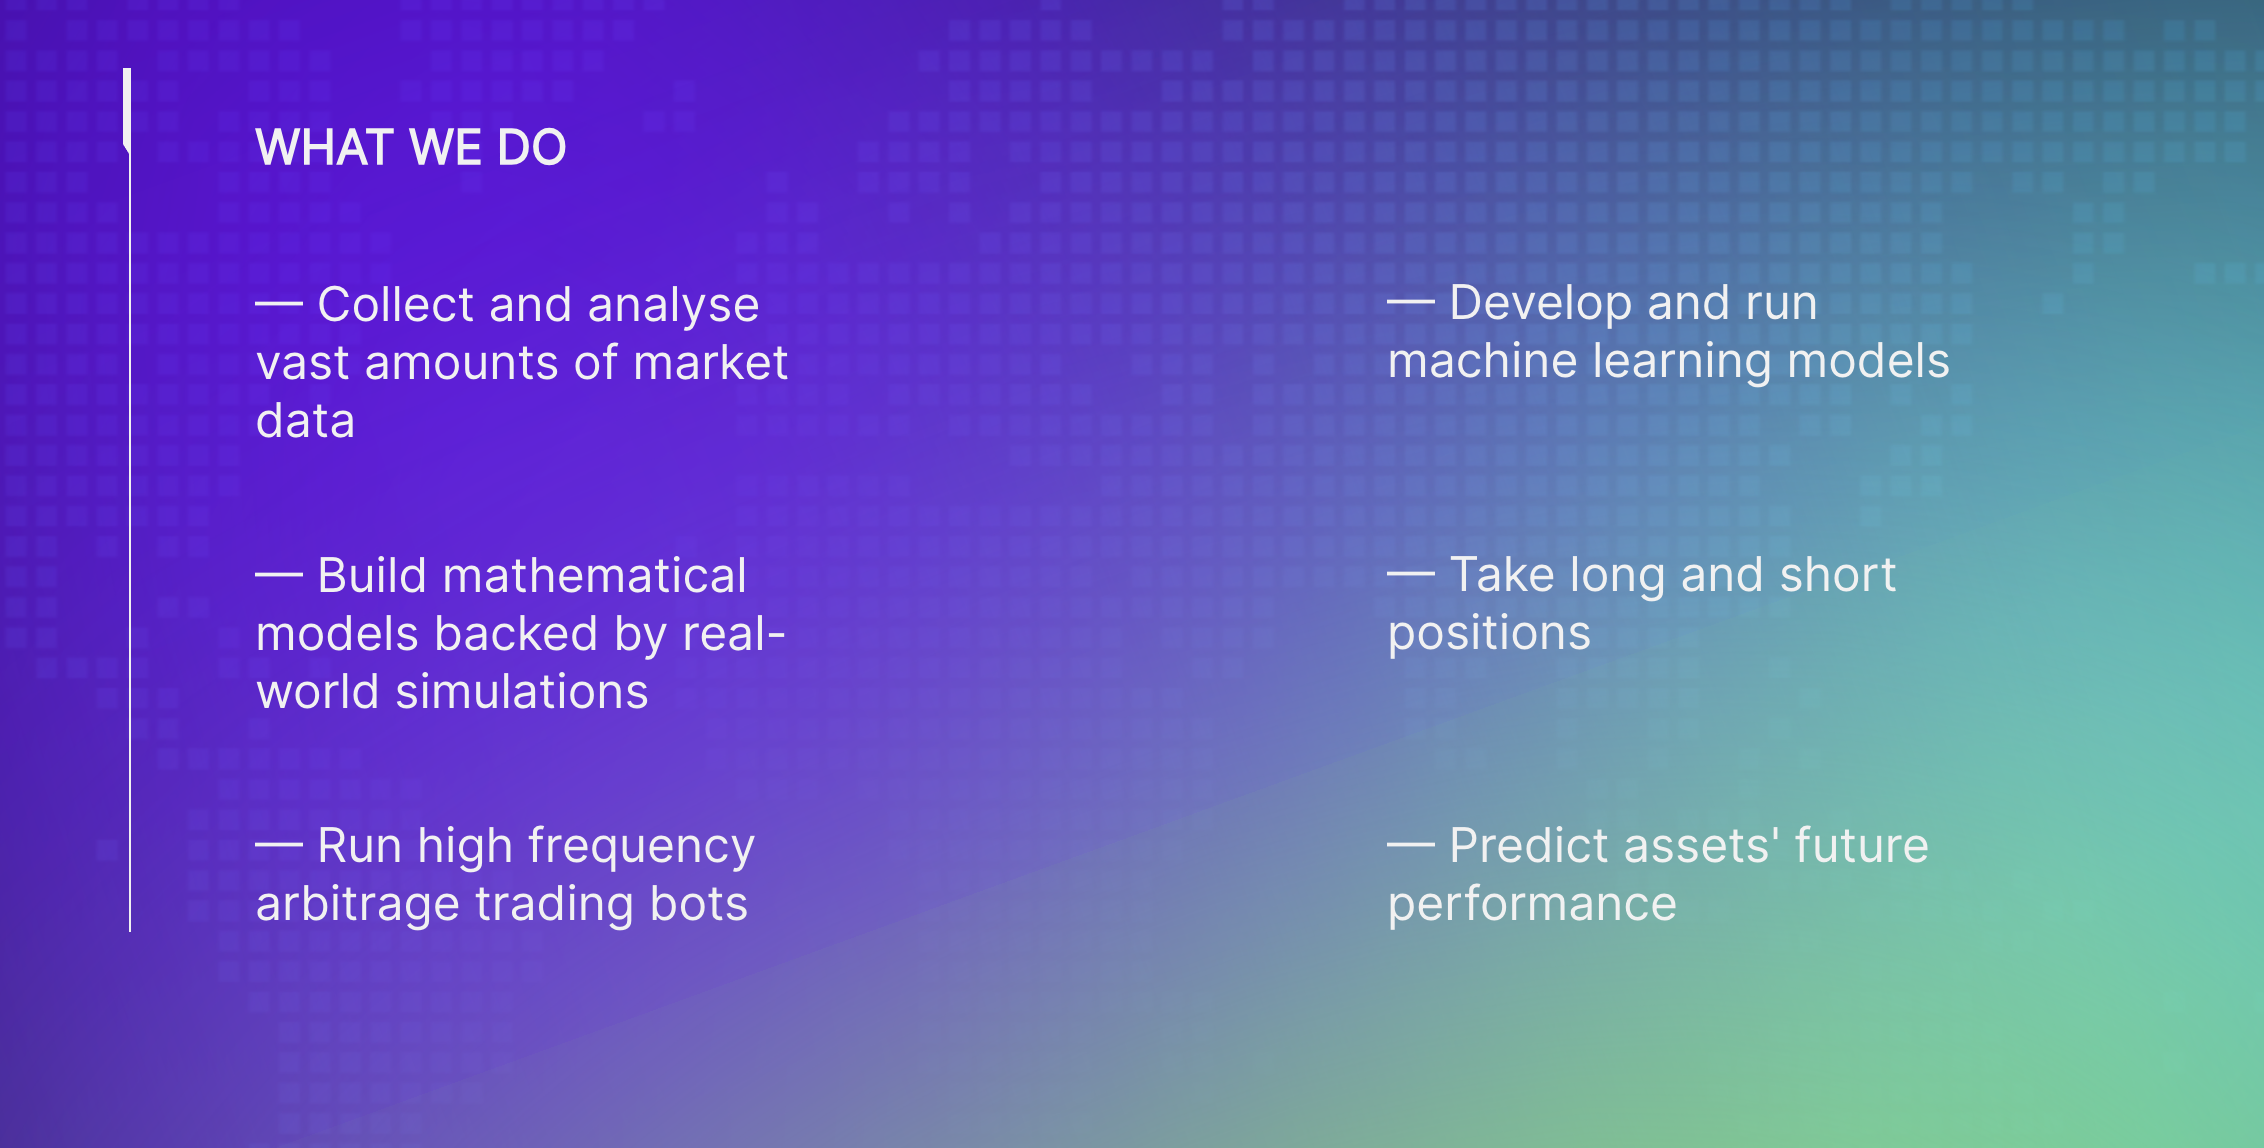
\includegraphics[scale=0.3]{resources/whatwedo.png}
    \label{img:whatwedo}
  \end{figure}
\end{frame}

\begin{frame}{Laiko juosta}
  Darbas tiek „Humbility“, tiek universitete yra tęstinis ir susijęs su ta pačia tema.

    % Humbilityje dirbu nuo x
  % o praktikoje aprasau darbą dvidesim treciu metu rugsejo iki lapkricio - kur darbas susietas su likvidacijomis
  % siu metu sausi pristaciau kursini darba, kurio tema x
  % tai buvo mano paties noras toliau pasikrapstyti su likvidacimo algoritmu ir pabandyti ji patobulinti

  \begin{itemize}
    \item \textbf{2021-10}: Pradėjau dirbti „Humbility“ įmonėje.
    \item \textbf{2023-09}: Pradėjau diegti likvidacijų mechanizmą.
    \item \textbf{2023-11}: Paleistas pirminis likvidacijų mechanizmo variantas.
    \item \textbf{2025-01}: Pristačiau kursinį darbą tema „Likvidavimo algoritmo tobulinimas perviršinio užstato skolinimo protokoluose“.
    \item \textbf{2025-06}: Baigiamajame bakalauro darbe pristatysiu šio darbo tęsinį ir tolesnius patobulinimus.
  \end{itemize}
\end{frame}


  % pirma rasta slacke https://bscscan.com/tx/0x6a26a2cd167eb06499f8a921c02449ee7fafaaceef0798af0ca592abd062accb
  % pirma paloginta i lenta https://bscscan.com/tx/0x3a651f15c75fff0630f44c8f39ac8307e2b98d2f0af75c52dc99d0c29826e30f

  

% 2188
% 1117911.3495707351
% 11151.73878648408
% 2025-04-30 21:40:19.000 +0300

\begin{frame}{Praktika}
  \begin{block}{Tema}
    Programų, skirtų prekiauti kripto valiutas, kūrimas, tobulinimas ir testavimas, naudojant Go ir Rust programavimo kalbas
  \end{block}
  
  Užduotys:
  \begin{enumerate}
    \item Įgyti praktinių žinių apie Go ir Rust bibliotekas, reikalingas vykdyti kripto valiutų
    prekybą.
    \item Susipažinti su programine įranga, kurią kripto valiutų prekybos ir stebėjimo tikslais naudoja įmonė.
    \item Kurti kripto valiutų prekiavimui programas ir tobulinti jas.
    \item Testuoti sukurtas ir/arba atnaujintas programas.
  \end{enumerate}
\end{frame}


% Konkreciai pasirinkau aprasyti darba su likvidacijomis
\begin{frame}{Naujas funkcionalumas - likvidacijos}
  % kas yra likvidacijos
  \textbf{Likvidacija} - saugumo priemonė, skirta užtikrinti, kad skolininkas laikytųsi savo įsipareigojimų.
  \begin{enumerate}
    \item Vartotojas į protokolą įneša turtą (pvz., ETH), kuris veikia kaip paskolos užstatas. Šis turtas turi turėti didesnę vertę nei paskola.
    %  – t. y. paskola yra perviršinio užstato
    \item Remiantis LTV (Loan-to-Value) riba, vartotojas gali skolintis tam tikrą sumą (pvz., 75\% nuo įkeisto turto vertės).
    \item Jeigu įkeisto turto vertė sumažėja (pvz., ETH kaina krinta), LTV santykis pradeda artėti prie rizikingos ribos.
    \item Kai paskolos LTV peržengia likvidacijos ribą, paskola tampa likviduotina. Tai reiškia, kad trečiosios šalys (likvidatoriai) gali pradėti išpirkti dalį užstato, kad sumažintų riziką protokolui.
    \item Likvidatoriai perima dalį užstato su nuolaida. Ši paskata motyvuoja juos aktyviai sekti paskolas ir jas likviduoti.
  \end{enumerate}
\end{frame}

\begin{frame}{Venus protokolas}
  \begin{itemize}
    \item Tuo metu tik Binance Smart Chain (BSC) blogų grandinėje.
    \item Įnešus turtą, vartotojas gauna vTokens (pvz. vBNB), kurie atspindi jo poziciją ir kaupia palūkanas.
  \end{itemize}

  \begin{figure}[H]
    \centering
    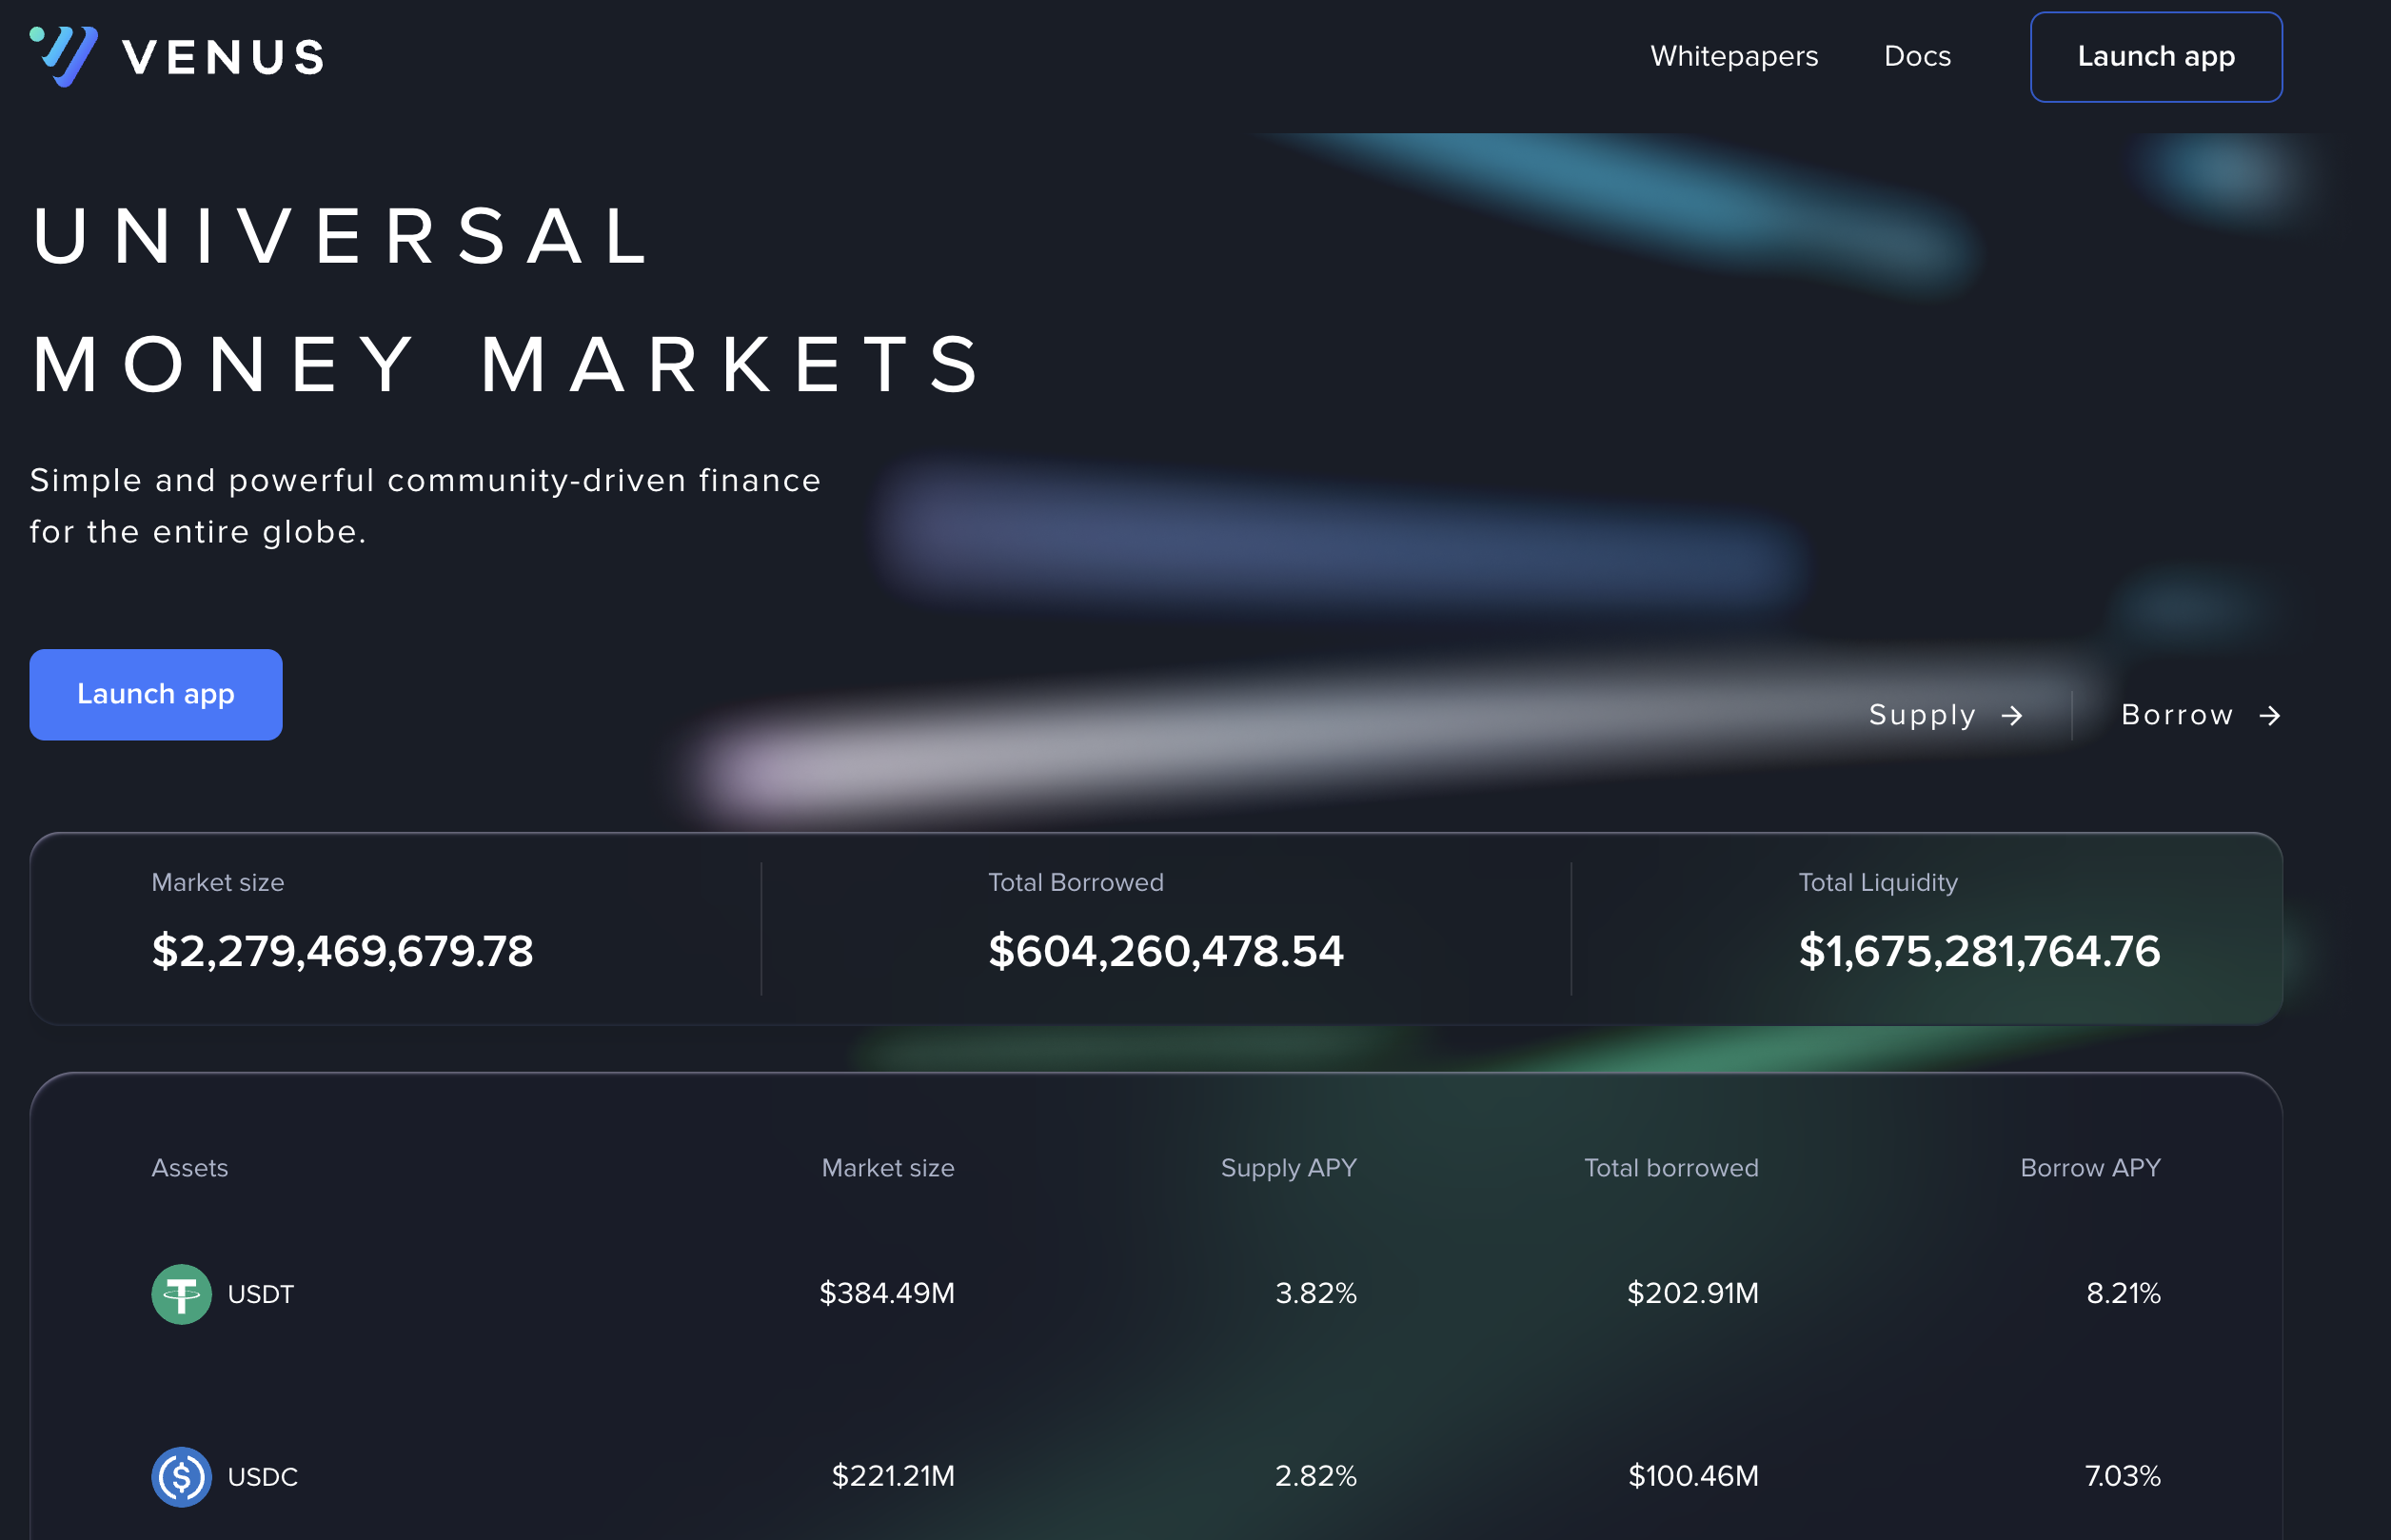
\includegraphics[scale=0.19]{resources/venus.png}
    \caption{Venus puslapis. https://venus.io}
    \label{img:venus}
  \end{figure}
\end{frame}

\begin{frame}{Nagrinėjimas}
  \begin{enumerate}
    \item Išnagrinėtas likvidavimo proceso mechanizmą skaitant venus kodą.
    \item Išsiaiškinta, kad skolininkų sarašą reikia gauti patiems nuskanavus visa bloku grandinę.
    \item Venus pasikliauna Chainlink orakulų paslauga. Žiūrėta kaip veikia jų mechanizmas.
    \item Konkurentų analizė. Norint būti pirmais likvidatoriais reikia mokėti reaguoti į tranzakcijas, kurios greitu metu pakeis valiutų vertes.
  \end{enumerate}
\end{frame}

\begin{frame}{Sprendimai}
  \begin{enumerate}
    \item C\# kalba parašyta aplikacija, renkanti duomenis apie skolininkus iš blokų grandinės (\textasciitilde{}1 000 eilučių).
    \item Golang kalba sukurtas servisas, kuris renka detalią informaciją apie skolininkus ir apskaičiuoja jų pozicijų „sveikumą“ (\textasciitilde{}15 000 eilučių).
    \item Pasinaudota esama infrastruktūra bei kodu, leidžiančiu greitai sužinoti apie naujai atsiradusius blokus ir pavienes tranzakcijas, kurios bus įtrauktos į blokus.
    \item Taip pat pritaikyta esama arbitražo paieškos sistema, skirta valiutų keitimo rinkoms. Pridėjus likvidavimo galimybes, išplėstas ieškomų galimybių spektras.
    \item Solidity kalba realizuotas likvidacijos vykdymas tiesiogiai blokų grandinėje (\textasciitilde{}200 eilučių).
  \end{enumerate}
\end{frame}

\begin{frame}{Likvidacijos pavyzdys}
  \begin{figure}[H]
    \centering
    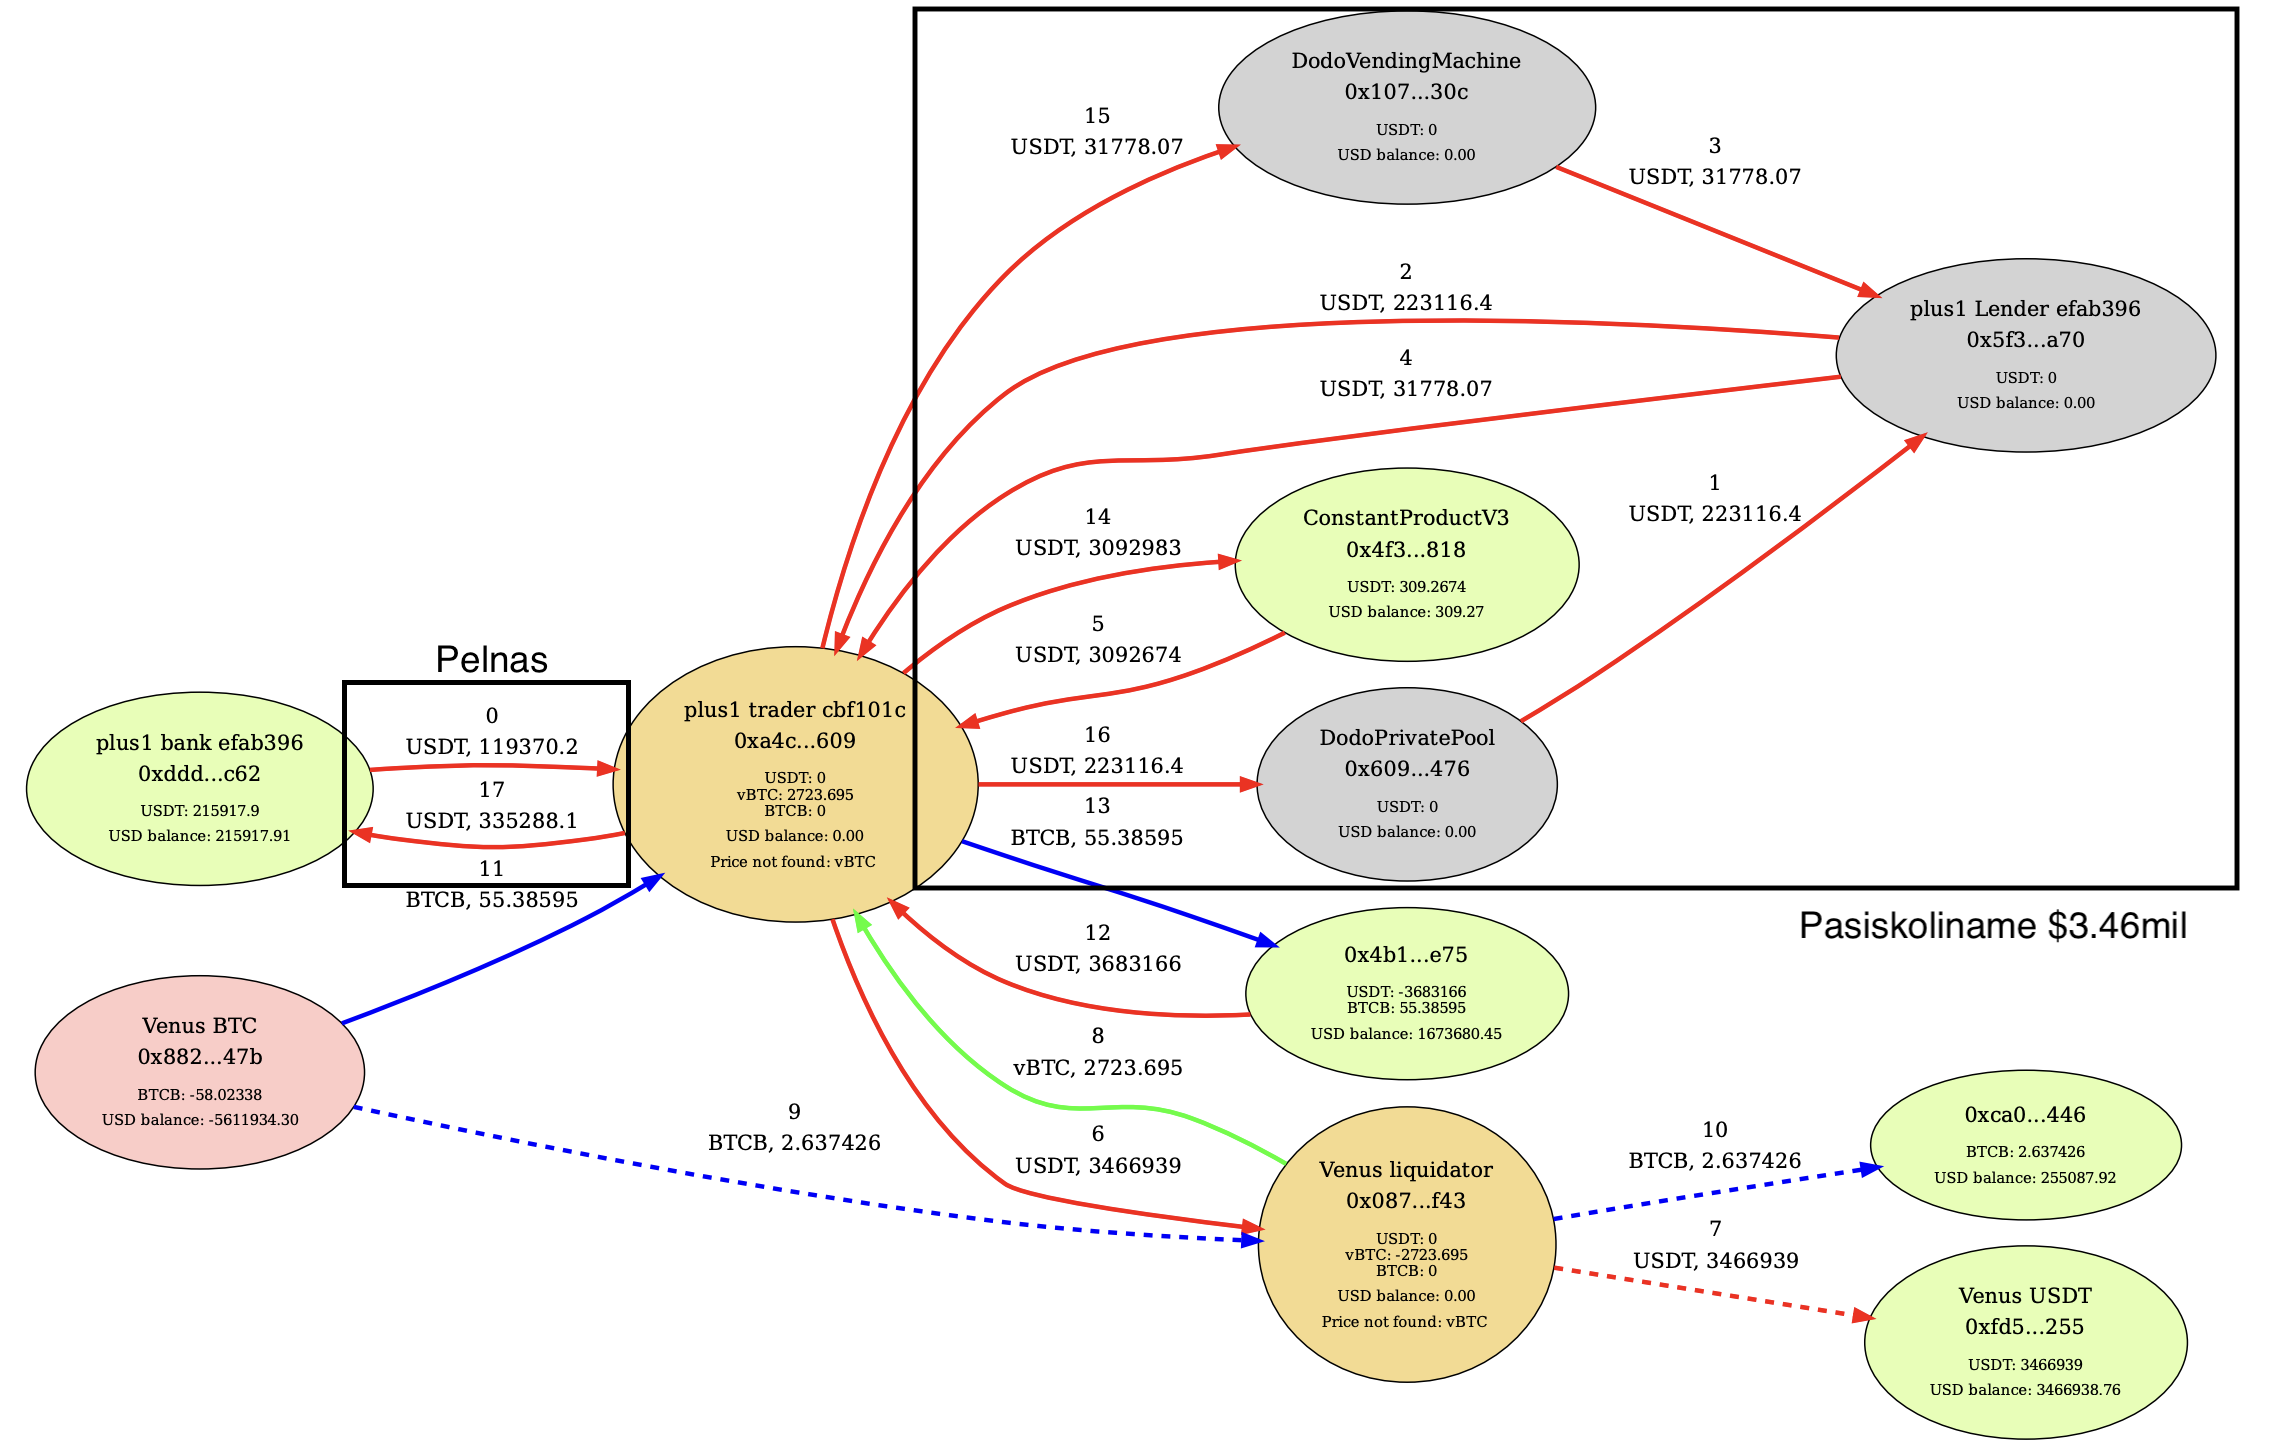
\includegraphics[scale=0.28]{resources/likvidacija.png}
    \caption{\$216 000 pelno likvidacija}
    \label{img:likvidacija}
  \end{figure}
\end{frame}

% Integruojant likvidacijos algoritmą į arbitražo sistemą, buvo susidurta su rimta našumo problema. Kadangi aktyvių skolininkų kiekis siekia dešimtis tūkstančių, kiekvienas valiutos kainos pokytis reikalauja peržiūrėti visų skolininkų pozicijas ir perskaičiuoti jų sveikumo koeficientą ($HF$), siekiant nustatyti ar pozicija tampa likviduojama. Šis procesas tapo akivaizdžiai per lėtas realaus laiko sistemai, kur kainos nuolat kinta.

% Siekiant šią problemą išspręsti, buvo sukurta specializuota duomenų struktūra – \texttt{zeroCenteredSet}. Šios struktūros principas remiasi tuo, kad kiekvienas skolininkas, priklausomai nuo turimų valiutų ir jų užstato santykio, yra priskiriamas prie tam tikros vietos skirtingose valiutų skalėse. Kiekviena tokia skalė yra centrinė pagal pradinę valiutos kainą ir išsiplečia tiek į teigiamą, tiek į neigiamą pusę – t. y. skalė yra simetriška aplink nulį.

% Kiekvieno skolininko pozicijos vieta šioje skalėje nusako, kokio dydžio kainos pokytis konkrečiai valiutai reikalingas, kad ta pozicija taptų likviduojama. Kai valiutos kaina keičiasi, apskaičiuojamas kainos pokytis nuo pradinės (ref) reikšmės, ir struktūra leidžia greitai išrinkti tik tuos skolininkus, kuriems šis pokytis reikšmingas. Taip eliminuojama būtinybė tikrinti visų skolininkų pozicijas, kas leidžia drastiškai sumažinti perskaičiavimų kiekį.

% \texttt{zeroCenteredSet} struktūra tapo esmine sistemos dalimi, leidžiančia užtikrinti greitą reagavimą į rinkos pokyčius ir išlaikyti sistemą efektyvią net ir esant itin didelei aktyvių paskolų bazei.

\begin{frame}{Našumo problema ir sprendimas}
  \begin{itemize}
    \item BSC grandinėje yra apie 164 000 potencialių Venus skolininkų.
    \item Nauji blokai atsiranda kas 3 sekundes.
    \item Norint suspėti likviduoti po valiutos kainos pokyčio, būtina patekti į kelių milisekundžių laiko langą.
    \item Problema - gavus atnaujintą valiutos kainą, visų skolininkų likvidumo perskaičiavimas užtrunka kelias sekundes.
  \end{itemize}

  \begin{figure}[H]
    \centering
    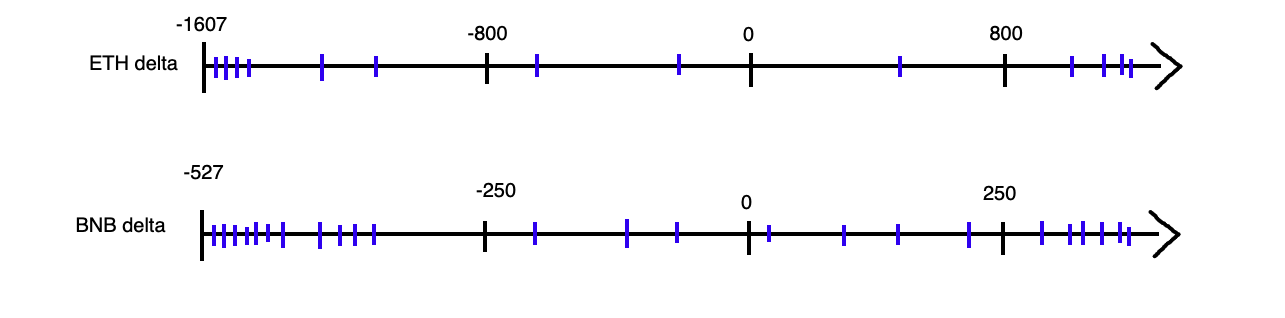
\includegraphics[scale=0.28]{resources/zerocent.png}
    \caption{Skolininkai išrikiuojami pagal kainos pokytį, reikalingą jų pozicijai tapti likviduotina}
    \label{img:zerocent}
  \end{figure}
\end{frame}

\begin{frame}{Nauda įmonei}
  Nuo 2024-02:
  \begin{itemize}
    \item Atliktos apie 2 200 likvidacijų.
    \item Įgyta daugiau nei \$1 000 000 pelno.
  \end{itemize}
\end{frame}

\begin{frame}{Rezultatai}
  \begin{itemize}
    \item Išanalizuotas \textit{Venus} paskolų protokolo veikimas ir sukurti algoritmai, leidžiantys automatiškai nustatyti likviduojamas pozicijas bei vykdyti pelningą likvidaciją.
    \item Integruotas likvidacijos algoritmas į esamą arbitražo sistemą, išplečiant jos funkcionalumą, kas suteikia galimybę pasiekti platesnį rinkų pasirinkimą, leidžiantį rasti daugiau valiutos keitimo kelių ir, atitinkamai, didesnę galimybę generuoti pelną per arbitražą.
  \end{itemize}
\end{frame}

% vakar siek tiek clickinau Venus, lending protocol BSC:
% gali kaip skolintis ir kaip collateral naudot didesnius tokenus. cia sarasas: https://app.venus.io/
% pvz kaip collateral uzstates BUSD gauni 2.6%, o pasiskolines BNB moki tik 1.59%, tai cia atrodo, kad turi BNB, kuriuos gali naudot ir eini i pliusa
% liquidation riba yra 80% collateral vertes
% UI suggestina skolintis ne daugiau nei 64% collateral vertes (tai turi 16% iki kol prasides likvidacija). sitie % gali skirtis nuo koki collateral naudoji
% likvidatorius likvidavimo metu padengia tavo skola ir pasiima 10% tavo collateral. kiek supratau, jei tik biski kerta 80% riba, tai negali visos tavo pozicijos likviduot, bet per daug nesigilinau i sita
% kaina ima is Oracles, jei tiksliau, man atrodo Chainlinko. bet situo mechanizmu irgi daugiau nesidomejau
% BSC likvidaciju pasitaiko kasdien, bet labai mazai. jas galim nesunkiai paziuret per Dune pasiquerinus liquidateBorrow logus


\begin{frame}
  \centering
  \Large Klausimai?
\end{frame}

\end{document}
